The goal of this project is to introduce Apache Spark in these NGS Pipelines in order to improve their efficiency. Here will be exposed the execution times of tools with different Spark and hardware configurations. 



\section{Local Mode}
As mentioned in previous chapters, the Preprocessing phase is the most time and resource consuming, with some numbers will be expressed the different execution times between the three phases.

\subsection{Preprocessing 6 genomes}
In Tables \ref{BWA_6_16} \ref{BQSR_6_16} \ref{HC_6_16} are listed the execution times of the preprocessing phase using 6 input samples, reporting the Spark configuration parameters too. The first step is the conversion through \textit{FatqToSam}: since that it is a \textit{Sparkified} tool, it benefits from only the cores of the host machine. Indeed while it takes 46 minutes to process an only genome, processing 6 genomes takes only 70 minutes on a single VM, applying each of the 6 conversions in parallel.\newline
As exposed in previous chapters, GATK Spark tools are meant to process a sample for each, so with a first \textit{for loop} have been executed the BwaAndMarkDuplicatesPipelineSpark on each input sample; each of the generated output has been used as input of \textit{for loop} of BQSRPipelineSpark and the same thing for HaplotypeCallerSpark. This means that the preprocessing phase for 6 samples lasted 3695,31 minutes (obtained summing the execution times of the 3 tables).\newline
Moreover this computation has been executed one more time, with a Spark parameters tuning, with results observable in Tables \ref{BWA_6_8} \ref{BQSR_6_8} \ref{HC_6_8}. By simply summing the execution times of these tables (as already done previously), we obtain 3511,7 minutes. This means that by simply tuning Spark parameters and using the same VM is possible to obtain some speed-up. Even comparing, for example, the execution times of BwaAndMarkDuplicatesPipelineSpark in Tables \ref{BWA_6_16} and \ref{BWA_6_8} it is observable that the time values reported in the second configuration are better than the first one. It is the same even for BQSRPipelineSpark, while HaplotypeCallerSpark is quite unpredictable: indeed looking at Charts \ref{cht:preprocessing16} \ref{cht:preprocessing8}, HaplotypeCallerSpark shows a strange behaviour, since in certain executions took less time with bigger size samples than smaller ones.
\\[1\baselineskip]
The analysis performance expressed in this subsection was conducted through GATK 4.0 BETA, when it was not an official release.

\subsection{Spark parameters tuning}
So it is worth to do some performance analysis on Spark parameters for these tools, due to find the best configuration. In Tables \ref{BWA_bench} \ref{BQSR_bench} \ref{HC_bench} are respectively reported BwaAndMarkDuplicatesPipelineSpark, BQSRPipelineSpark and HaplotypeCallerSpark  benchmarking with different Spark parameters, using the same input sample and same VM.\newline
For BwaAndMarkDuplicatesPipelineSpark seems that using driver-memory 10GB num-executors 4 executor-cores 2 executor-memory 8 is obtainable the best execution time. Even if has been executed two times with these parameters and obtained a little bit slower performance (to demonstrate that these processes are not perfectly time predictable).
\\[1\baselineskip]
Even here analysis performance was conducted through GATK 4.0 BETA.

\subsection{Variant Discovery and Call-set Refinement}
Comparing these numbers with the execution times reported for Variant Discovery and Call-set Refinement makes understandable the great difference of time executions between these three phases. In Tables \ref{vd} \ref{cr} are reported the execution times of the simple tools (not \textit{Sparkified}) respectively of the Variant Discovery and Call-set Refinement phase. These tools used the output files generated by the HaplotypeCallerSpark on the 6 samples (\ref{HC_6_16}), because the GenotypeGVCFs require more input files, with only one does not work. Has been noticed that 6 is a good number of input samples and in this this condition the tool works.\newline
With the \textit{Sparkified} version, which gathers respectively the tools of Variant Discovery and Call-set refinement (listed in Tables \ref{vd} and \ref{cr}), was measured respectively 13,82 and 31,37 minutes. Comparing these values with the previous calculated of preprocessing, through the Chart \ref{cht:pvc} is possible to have an idea of the different execution times.

\subsection{Scale up}
In order to introduce parallelism in this pipeline (or in general) there are two approaches: \textit{scale up} and \textit{scale out}.\newline
With the first approach the work load is distributed on more virtual cores of the same VM, which means using VM with better hardware resources. In the second one the work load is distributed on hardware resources of different VMs, a computer cluster that cooperate to processing data. This is possible due to sharing intermediate results of the computation that lead to the final result. This data sharing between nodes in the same cluster is possible through networking and shared file system, which allow the nodes of the cluster to communicate each other. The inconvenient of this approach is the introduction of overhead, because these intermediate results must be communicated over the network (even if it is a local network). Scaling-up avoids these delays, and with the same combined hardware resources, this approach gives better results. So executing BwaAndMarkDuplicatesPipelineSpark on a VM with 16 cores and 110 GB of RAM takes 129,29 minutes. While BQSRPipelineSpark takes 36,62 minutes, as reported in Chart \ref{cht:scale-up}. Comparing these numbers with values reported in Tables \ref{BWA_6_16} \ref{BQSR_6_16}, we almost have an ideal speed-up, since doubling the number of cores, almost halves the execution time (in next section will be discussed the scale out approach).\newline
While HaplotypeCallerSpark with 16 cores took more time. Analysing the log output of the execution, there is a warning that explain the reason of so much long execution time:
\begin{lstlisting}[language=Java,caption={Missing AVX instruction}]
WARN  PairHMM - ***WARNING: 
Machine does not have the AVX instruction set support needed for
the accelerated AVX PairHmm. 
Falling back to the MUCH slower LOGLESS_CACHING implementation!
\end{lstlisting}
It seems that resizeing the Azure VM to 16 cores, provides a different CPU. This one is not compatible with HaplotypeCallerSpark requirements and so it uses a much slower implementation.\newline
Moreover these tools have been executed even on a VM with 32 cores and 120 GB of RAM, reporting all these results of scaleing up in Chart \ref{cht:scale-up}. As observable from this chart, using 32 cores lead to an unpredicted behaviour: instead to further decrease the execution time of the tool, this value just increased instead. Probably this is due to the limit of obtainable speed-up with this configuration. Further analysis may be required to understand the reason of this behaviour. 
\\[1\baselineskip]
Here was used GATK 4.0.2.0 release. It is interesting to notice that using this release for previous exposed cases changes their execution times, increasing this value. They are still working on these tools and there are still known issues to resolve.

\section{Cluster Mode}
As mentioned in Clustering chapter, finding the right configuration was pretty hard. After finding the right parameter in a GitHub issue, the pipeline have been executed on a cluster of two VMs. The results are observable in Table \ref{cluster} for BwaAndMarkDuplicatesPipelineSpark. Unfortunately there was still some unresolved problem in executing HaplotypeCallerSpark.\newline
Anyway from the reported results, is possible to notice that comparing the second row with results reported in Table \ref{BWA_bench} (which means using of VMs with same hardware, changing only the number of VMs) have been obtained a certain speed-up, passing from about 250 minutes to 169,29. Comparing this value with the 129,29 minutes obtained scaling up, confirms what exposed previously. In both cases have been used 16 cores and 110 GB of RAM, but in the scale-up the resources were on a single VM, giving better performance. In the scale-out these resources have been distributed in 2 nodes (other results are observable at Chart \ref{cht:scale-out}).\newline
While analysing the result of the first row of Table \ref{}, in which has been used a 2 Nodes Cluster with double hardware resources per VM, which means each VM has 16 cores and 110 GB of RAM, gives even an higher speed-up, with 94,63 minutes.
\\[1\baselineskip]
Here was used GATK 4.0.2.0 release too.

\section{Microsoft Genomics}
Microsoft give the possibility to execute their genomic pipeline described in their paper \cite{MicrosoftGenomics}. Their approach is to run separately each genome on a single high-capacity virtual machine, to maximize throughput and minimize communication and storage overhead within each run. So instead of using a cluster which would introduce delays due to network and disk accesses, using an only high-capacity virtual machine avoids these delays. Their pipeline arrives until the Haplotype Caller (in other words is only the Preprocessing phase described in this thesis), without Variant Calling and Call-set Refinement phases. Moreover has an option to produce a gVCF file, which can be merged across multiple samples for joint genotyping, but for this moment it is not available. Only VCF files are produced at the end of this process, while the pipeline implemented in this project produces gVCF files.\newline
The key difference between a regular VCF and a gVCF is that the gVCF has records for all sites, whether there is a variant call there or not. The goal is to have every site represented in the file in order to do joint analysis of a cohort in subsequent steps. The records in a gVCF include an accurate estimation of confidence in the determination that the sites are homozygous-reference or not. This estimation is generated by the HaplotypeCaller's built-in reference model \cite{gVCF}.\newline
Analysing their performance, processing the sample PFC\_0028 reported in Tables \ref{BWA_bench} \ref{BQSR_bench} \ref{HC_bench} takes only 76,88 minutes. Unfortunately they do not provide info about the VM specifics which process this sample. 
\subsection{Pricing Analysis}
What they provide is a \href{https://azure.microsoft.com/en-en/pricing/details/genomics/}{pricing rate}, where is reported the \pounds 0.217/gigabase pricing. Which means that processing the 6 samples exposed in subsection \textit{Preprocessing 6 genomes} through the Microsoft Genomics pipeline costs \pounds 18.61, since that should be processed roughly 85 gigabases. Making a comparison with the pipeline implemented in this project, for processing the first mentioned 6 genomes were necessary 3511,7 minutes on a VM with 8 cores and 55 GB of RAM, which pricing is of \pounds 354,89/month. With some calculations, processing 6 genomes costs \pounds28,84 here. So the Microsoft Genomics pipeline is even cheaper.

%****************************************************%
\begin{table}[h]
	\caption{BwaAndMarkDuplicatesPipelineSpark Execution Times~\label{BWA_6_16}}
	\begin{center}
		\begin{tabular}{| m{5em} | m{5em} | m{3em} | m{4em} | m{4em} | m{5em} | m{4.5em} | m{3em} |}
    		\hline
    		Tool & Input & driver-memory & num-executors & executor-cores & executor-memory & VM & Time (m) \\ \hline
		    BWA\&MD & PFC\_0033 15,9 GB & 20 GB & 2 & 4 & 16 GB & 8 Cores 55g RAM & 306,57 \\ \hline
			BWA\&MD & PFC\_0032 14,4 GB & 20 GB & 2 & 4 & 16 GB & 8 Cores 55g RAM  & 270,10 \\ \hline
			BWA\&MD & PFC\_0031 10,8 GB & 20 GB & 2 & 4 & 16 GB & 8 Cores 55g RAM  & 194,21 \\ \hline
			BWA\&MD & PFC\_0030 13,2 GB& 20 GB & 2 & 4 & 16 GB & 8 Cores 55g RAM  & 261,93 \\ \hline
			BWA\&MD & PFC\_0029 13 GB & 20 GB & 2 & 4 & 16 GB & 8 Cores 55g RAM  & 264,71 \\ \hline
			BWA\&MD & PFC\_0028 14,2 GB & 20 GB & 2 & 4 & 16 GB & 8 Cores 55g RAM  & 282,81 \\ \hline
    	\end{tabular}
    \end{center}
\end{table}
%****************************************************%
\begin{table}[h]
	\caption{BQSRPipelineSpark Execution Times~\label{BQSR_6_16}}
	\begin{center}
		\begin{tabular}{| m{5em} | m{5em} | m{3em} | m{4em} | m{4em} | m{5em} | m{4.5em} | m{3em} |}
    		\hline
    		Tool & Input & driver-memory & num-executors & executor-cores & executor-memory & VM & Time (m) \\ \hline
		    BQSR & PFC\_0033 15,9 GB & 20 GB & 2 & 4 & 16 GB & 8 Cores 55g RAM & 95,91 \\ \hline
			BQSR & PFC\_0032 14,4 GB & 20 GB & 2 & 4 & 16 GB & 8 Cores 55g RAM  & 78,66 \\ \hline
			BQSR & PFC\_0031 10,8 GB & 20 GB & 2 & 4 & 16 GB & 8 Cores 55g RAM  & 60,38 \\ \hline
			BQSR & PFC\_0030 13,2 GB& 20 GB & 2 & 4 & 16 GB & 8 Cores 55g RAM  & 72,55 \\ \hline
			BQSR & PFC\_0029 13 GB & 20 GB & 2 & 4 & 16 GB & 8 Cores 55g RAM  & 76,92 \\ \hline
			BQSR & PFC\_0028 14,2 GB & 20 GB & 2 & 4 & 16 GB & 8 Cores 55g RAM  & 73,53 \\ \hline
    	\end{tabular}
    \end{center}
\end{table}
%****************************************************%
\begin{table}[h]
	\caption{HaplotypeCallerSpark Execution Times~\label{HC_6_16}}
	\begin{center}
		\begin{tabular}{| m{5em} | m{5em} | m{3em} | m{4em} | m{4em} | m{5em} | m{4.5em} | m{3em} |}
    		\hline
    		Tool & Input & driver-memory & num-executors & executor-cores & executor-memory & VM & Time (m) \\ \hline
		    HC & PFC\_0033 15,9 GB & 20 GB & 2 & 4 & 16 GB & 8 Cores 55g RAM & 380,19 \\ \hline
			HC & PFC\_0032 14,4 GB & 20 GB & 2 & 4 & 16 GB & 8 Cores 55g RAM  & 296,59 \\ \hline
			HC & PFC\_0031 10,8 GB & 20 GB & 2 & 4 & 16 GB & 8 Cores 55g RAM  & 222,01 \\ \hline
			HC & PFC\_0030 13,2 GB& 20 GB & 2 & 4 & 16 GB & 8 Cores 55g RAM  & 226,70 \\ \hline
			HC & PFC\_0029 13 GB & 20 GB & 2 & 4 & 16 GB & 8 Cores 55g RAM  & 300,07 \\ \hline
			HC & PFC\_0028 14,2 GB & 20 GB & 2 & 4 & 16 GB & 8 Cores 55g RAM  & 231,47 \\ \hline
    	\end{tabular}
    \end{center}
\end{table}
%****************************************************%
\begin{chart}[!ht]
\centering
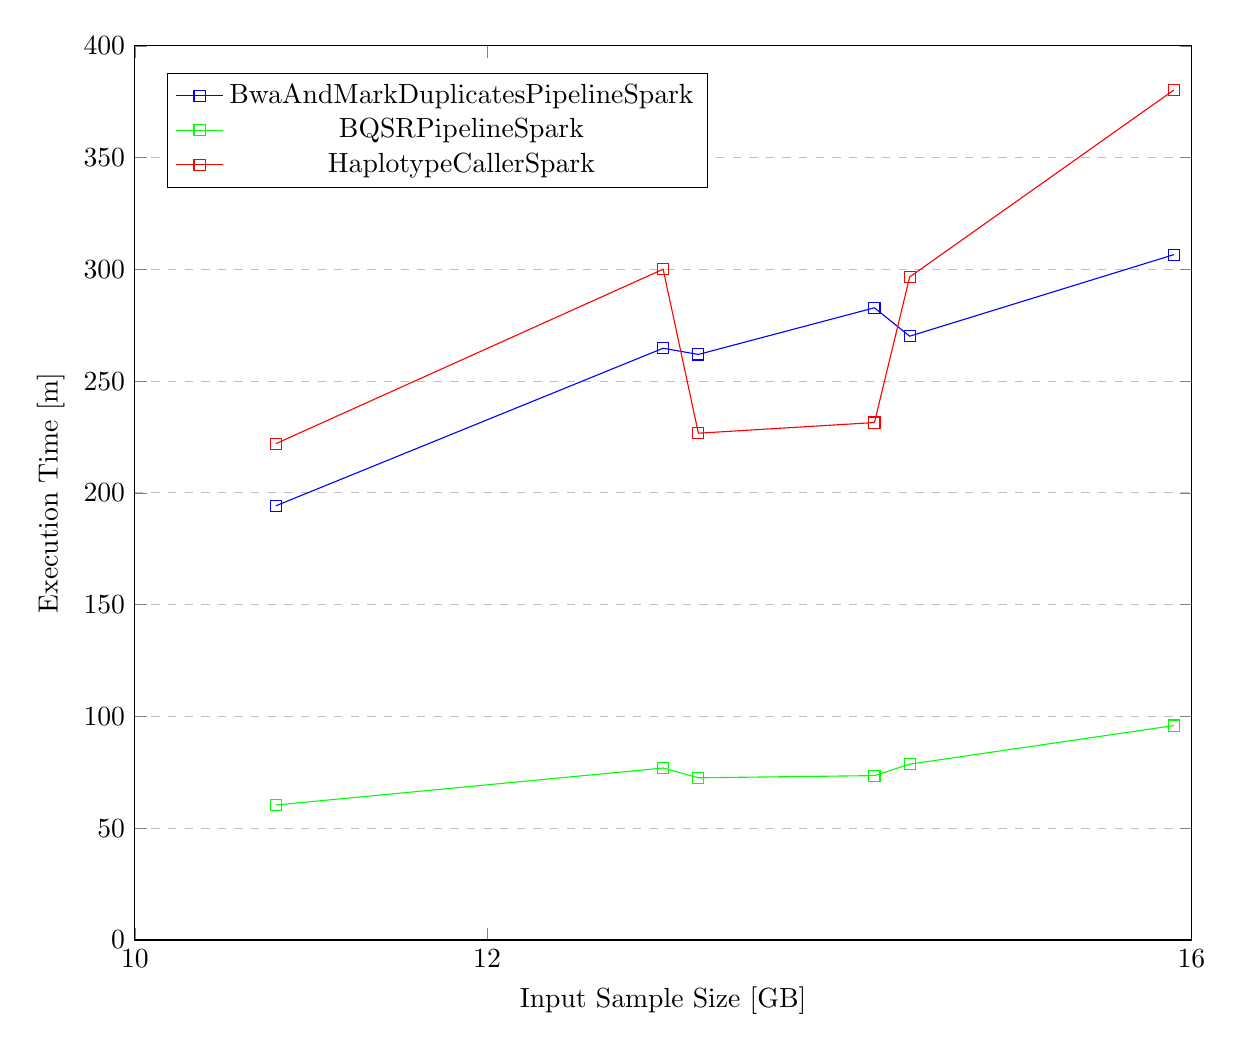
\begin{tikzpicture}
\pgfplotsset{width=15cm,compat=1.9}
\begin{axis}[
    title={},
    xlabel={Input Sample Size [GB]},
    ylabel={Execution Time [m]},
    xmin=10, xmax=16,
    ymin=0, ymax=400,
    xtick={10,12,16},
    ytick={0,50,100,150,200,250,300,350,400},
    legend pos=north west,
    ymajorgrids=true,
    grid style=dashed,
]
 
\addplot[ color=blue, mark=square, ]
    coordinates {
    (10.8,194.21)(13,264.71)(13.2,261.93)(14.2,282.81)(14.4,270.10)(15.9,306.57)
    };

\addplot[ color=green, mark=square, ]
    coordinates {
    (10.8,60.38)(13,76.92)(13.2,72.55)(14.2,73.53)(14.4,78.66)(15.9,95.91)
    };

\addplot[ color=red, mark=square, ]
    coordinates {
    (10.8,222.01)(13,300.07)(13.2,226.70)(14.2,231.47)(14.4,296.59)(15.9,380.19)
    };
\legend{BwaAndMarkDuplicatesPipelineSpark,BQSRPipelineSpark,HaplotypeCallerSpark}
\end{axis}
\end{tikzpicture}
\caption{Preprocessing of 6 samples in local-mode (8 Cores 55GB RAM) using Spark parameters: --driver-memory 20GB	--num-executors	2 --executor-cores	4 --executor-memory 16GB}\label{cht:preprocessing16}
\end{chart}
%____________________________________________________%
%____________________________________________________%
%____________________________________________________%
\begin{table}[h]
	\caption{BwaAndMarkDuplicatesPipelineSpark Execution Times~\label{BWA_6_8}}
	\begin{center}
		\begin{tabular}{| m{5em} | m{5em} | m{3em} | m{4em} | m{4em} | m{5em} | m{4.5em} | m{3em} |}
    		\hline
    		Tool & Input & driver-memory & num-executors & executor-cores & executor-memory & VM & Time (m) \\ \hline
		    BWA\&MD & PFC\_0033 15,9 GB & 20 GB & 4 & 2 & 8 GB & 8 Cores 55g RAM & 292,06 \\ \hline
			BWA\&MD & PFC\_0032 14,4 GB & 20 GB & 4 & 2 & 8 GB & 8 Cores 55g RAM  & 258,65 \\ \hline
			BWA\&MD & PFC\_0031 10,8 GB & 20 GB & 4 & 2 & 8 GB & 8 Cores 55g RAM  & 188,03 \\ \hline
			BWA\&MD & PFC\_0030 13,2 GB& 20 GB & 4 & 2 & 8 GB & 8 Cores 55g RAM  & 247,00 \\ \hline
			BWA\&MD & PFC\_0029 13 GB & 20 GB & 4 & 2 & 8 GB & 8 Cores 55g RAM  & 249,50 \\ \hline
			BWA\&MD & PFC\_0028 14,2 GB & 20 GB & 4 & 2 & 8 GB & 8 Cores 55g RAM  & 265,71 \\ \hline
    	\end{tabular}
    \end{center}
\end{table}
%****************************************************%
\begin{table}[h]
	\caption{BQSRPipelineSpark Execution Times~\label{BQSR_6_8}}
	\begin{center}
		\begin{tabular}{| m{5em} | m{5em} | m{3em} | m{4em} | m{4em} | m{5em} | m{4.5em} | m{3em} |}
    		\hline
    		Tool & Input & driver-memory & num-executors & executor-cores & executor-memory & VM & Time (m) \\ \hline
		    BQSR & PFC\_0033 15,9 GB & 20 GB & 4 & 2 & 8 GB & 8 Cores 55g RAM & 92,31 \\ \hline
			BQSR & PFC\_0032 14,4 GB & 20 GB & 4 & 2 & 8 GB & 8 Cores 55g RAM  & 77,08 \\ \hline
			BQSR & PFC\_0031 10,8 GB & 20 GB & 4 & 2 & 8 GB & 8 Cores 55g RAM  & 54,50 \\ \hline
			BQSR & PFC\_0030 13,2 GB& 20 GB & 4 & 2 & 8 GB & 8 Cores 55g RAM  & 69,45 \\ \hline
			BQSR & PFC\_0029 13 GB & 20 GB & 4 & 2 & 8 GB & 8 Cores 55g RAM  & 73,28 \\ \hline
			BQSR & PFC\_0028 14,2 GB & 20 GB & 4 & 2 & 8 GB & 8 Cores 55g RAM  & 72,25 \\ \hline
    	\end{tabular}
    \end{center}
\end{table}
%****************************************************%
\begin{table}[h]
	\caption{HaplotypeCallerSpark Execution Times~\label{HC_6_8}}
	\begin{center}
		\begin{tabular}{| m{5em} | m{5em} | m{3em} | m{4em} | m{4em} | m{5em} | m{4.5em} | m{3em} |}
    		\hline
    		Tool & Input & driver-memory & num-executors & executor-cores & executor-memory & VM & Time (m) \\ \hline
		    HC & PFC\_0033 15,9 GB & 20 GB & 4 & 2 & 8 GB & 8 Cores 55g RAM & 434,23 \\ \hline
			HC & PFC\_0032 14,4 GB & 20 GB & 4 & 2 & 8 GB & 8 Cores 55g RAM  & 260,60 \\ \hline
			HC & PFC\_0031 10,8 GB & 20 GB & 4 & 2 & 8 GB & 8 Cores 55g RAM  & 226,21 \\ \hline
			HC & PFC\_0030 13,2 GB& 20 GB & 4 & 2 & 8 GB & 8 Cores 55g RAM  & 186,72 \\ \hline
			HC & PFC\_0029 13 GB & 20 GB & 4 & 2 & 8 GB & 8 Cores 55g RAM  & 268,43 \\ \hline
			HC & PFC\_0028 14,2 GB & 20 GB & 4 & 2 & 8 GB & 8 Cores 55g RAM  & 195,69 \\ \hline
    	\end{tabular}
    \end{center}
\end{table}
%****************************************************%
\begin{chart}[!ht]
\centering
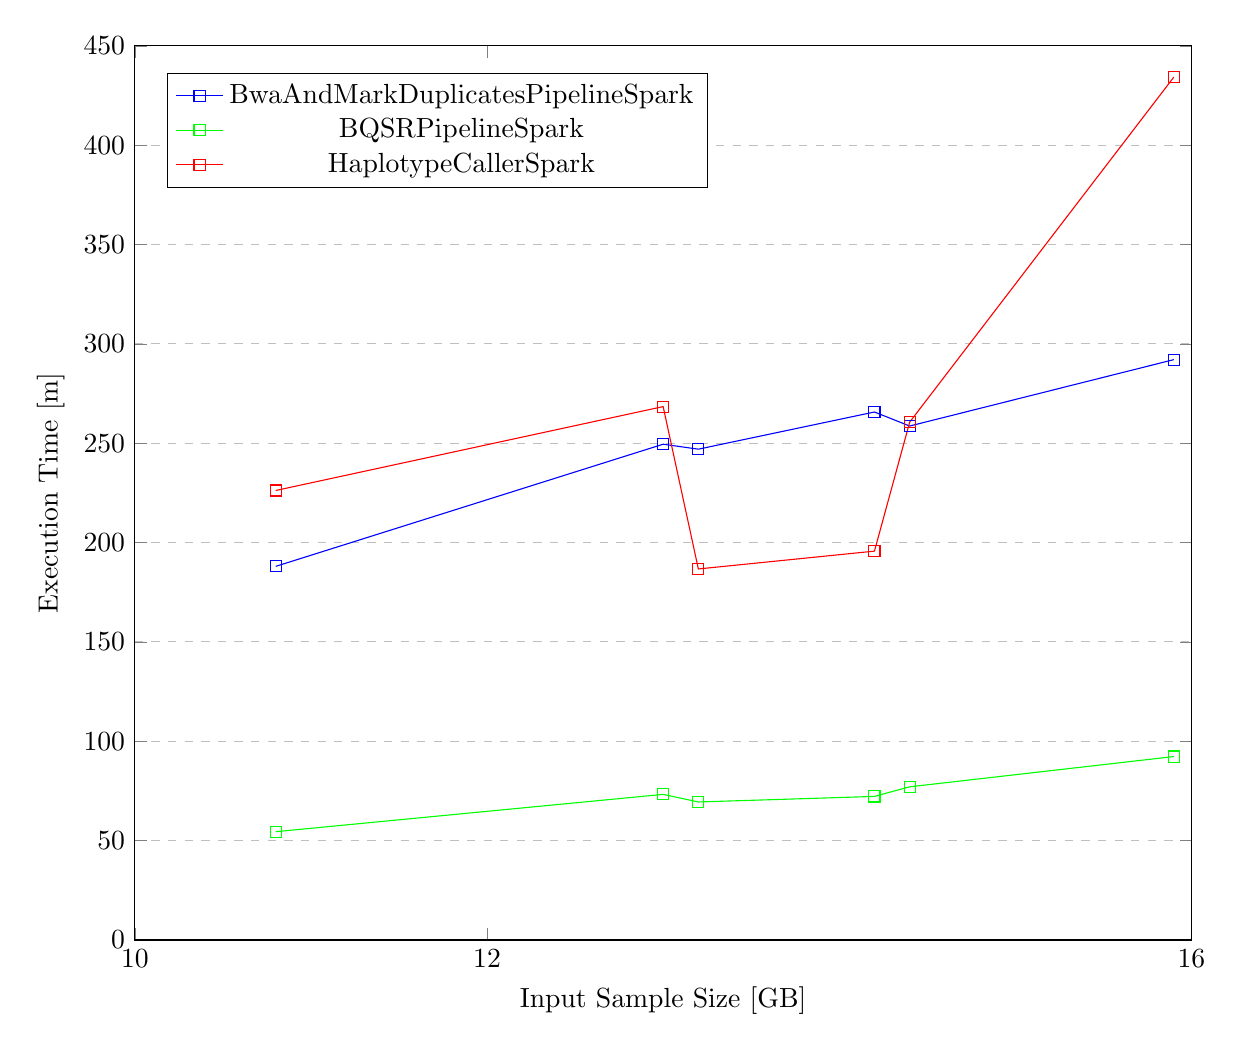
\begin{tikzpicture}
\pgfplotsset{width=15cm,compat=1.9}
\begin{axis}[
    title={},
    xlabel={Input Sample Size [GB]},
    ylabel={Execution Time [m]},
    xmin=10, xmax=16,
    ymin=0, ymax=450,
    xtick={10,12,16},
    ytick={0,50,100,150,200,250,300,350,400,450},
    legend pos=north west,
    ymajorgrids=true,
    grid style=dashed,
]
 
\addplot[ color=blue, mark=square, ]
    coordinates {
    (10.8,188.03)(13,249.50)(13.2,247.00)(14.2,265.71)(14.4,258.65)(15.9,292.06)
    };
\addplot[ color=green, mark=square, ]
    coordinates {
    (10.8,54.50)(13,73.28)(13.2,69.45)(14.2,72.25)(14.4,77.08)(15.9,92.31)
    };
\addplot[ color=red, mark=square, ]
    coordinates {
    (10.8,226.21)(13,268.43)(13.2,186.72)(14.2,195.69)(14.4,260.60)(15.9,434.23)
    };
\legend{BwaAndMarkDuplicatesPipelineSpark,BQSRPipelineSpark,HaplotypeCallerSpark}
\end{axis}
\end{tikzpicture}
\caption{Preprocessing of 6 samples in local-mode (8 Cores 55GB RAM) using Spark parameters: --driver-memory 20GB --num-executors 4 --executor-cores 2 --executor-memory 8GB}\label{cht:preprocessing8}
\end{chart}




\begin{table}[h]
	\caption{BwaAndMarkDuplicatesPipelineSpark Benchmarking~\label{BWA_bench}}
	\begin{center}
		\begin{tabular}{| m{5em} | m{5em} | m{3em} | m{4em} | m{4em} | m{5em} | m{4.5em} | m{3em} |}
    		\hline
    		Tool & Input & driver-memory & num-executors & executor-cores & executor-memory & VM & Time (m) \\ \hline
		    BWA\&MD & PFC\_0028 & 20 GB & 4 & 2 & 8 GB & 8 Cores 55g RAM & 270,27 \\ \hline
			BWA\&MD & PFC\_0028 & 10 GB & 4 & 2 & 8 GB & 8 Cores 55g RAM  & 251,8 \\ \hline
			BWA\&MD & PFC\_0028 & 10 GB & 4 & 2 & 8 GB & 8 Cores 55g RAM  & 258,3 \\ \hline
			BWA\&MD & PFC\_0028 & 10 GB & 2 & 4 & 8 GB & 8 Cores 55g RAM  & 255,74 \\ \hline
			BWA\&MD & PFC\_0028 & 10 GB & 2 & 4 & 8 GB & 8 Cores 55g RAM  & 254,91 \\ \hline
			BWA\&MD & PFC\_0028 & 10 GB & 8 & 1 & 6 GB & 8 Cores 55g RAM  & 281,85 \\ \hline
			BWA\&MD & PFC\_0028 & 5 GB & 4 & 2 & 12 GB & 8 Cores 55g RAM  & 279,18 \\ \hline
			BWA\&MD & PFC\_0028 & 5 GB & 4 & 2 & 8 GB & 8 Cores 55g RAM  & 264,99 \\ \hline
            
    	\end{tabular}
    \end{center}
\end{table}

\begin{table}[h]
	\caption{BQSRPipelineSpark Benchmarking~\label{BQSR_bench}}
	\begin{center}
		\begin{tabular}{| m{5em} | m{5em} | m{3em} | m{4em} | m{4em} | m{5em} | m{4.5em} | m{3em} |}
    		\hline
    		Tool & Input & driver-memory & num-executors & executor-cores & executor-memory & VM & Time (m) \\ \hline
		    BQSR & PFC\_0028 & 5 GB & 4 & 2 & 8 GB & 8 Cores 55g RAM & 71,66 \\ \hline
			BQSR & PFC\_0028 & 10 GB & 4 & 2 & 8 GB & 8 Cores 55g RAM  & 71,43 \\ \hline
			BQSR & PFC\_0028 & 10 GB & 8 & 1 & 6 GB & 8 Cores 55g RAM & 74,98 \\ \hline            
    	\end{tabular}
    \end{center}
\end{table}

\begin{table}[h]
	\caption{HaplotypeCallerSpark Benchmarking~\label{HC_bench}}
	\begin{center}
		\begin{tabular}{| m{5em} | m{5em} | m{3em} | m{4em} | m{4em} | m{5em} | m{4.5em} | m{3em} |}
    		\hline
    		Tool & Input & driver-memory & num-executors & executor-cores & executor-memory & VM & Time (m) \\ \hline
		    HC & PFC\_0028 & 10 GB & 8 & 1 & 6 GB & 8 Cores 55g RAM & 227,36 \\ \hline
			HC & PFC\_0028 & 10 GB & 4 & 2 & 8 GB & 8 Cores 55g RAM  & 230,7 \\ \hline
			HC & PFC\_0028 & 20 GB & 4 & 2 & 8 GB & 8 Cores 55g RAM  & 225,85 \\ \hline
			HC & PFC\_0028 & 20 GB & 2 & 4 & 8 GB & 8 Cores 55g RAM  & 191,49 \\ \hline
			HC & PFC\_0028 & 20 GB & 1 & 8 & 8 GB & 8 Cores 55g RAM  & 195,28 \\ \hline
			HC & PFC\_0028 & 20 GB & 2 & 4 & 16 GB & 8 Cores 55g RAM  & 194,07 \\ \hline
			HC & PFC\_0028 & 20 GB & 2 & 4 & 4 GB & 8 Cores 55g RAM  & 233,31 \\ \hline
            
    	\end{tabular}
    \end{center}
\end{table}


\begin{table}[h]
	\caption{Variant Discovery ~\label{vd}}
	\begin{center}
		\begin{tabular}{| m{12em} | m{11em} | m{8em} | m{5em} |}
    		\hline
    		Tool & Input & VM & Time (m) \\ \hline
		    GenotypeGVCFs & PFC(28-29-30-31-32-33) & 8 Cores 55g RAM & 9,47 + 8,38 \\ \hline
			VariantRecalibratorSNP & PFC(28-29-30-31-32-33) & 8 Cores 55g RAM  & 9,53 \\ \hline
			ApplyRecalibrationSNP & PFC(28-29-30-31-32-33) & 8 Cores 55g RAM  & 0,42 \\ \hline
			VariantRecalibratorINDEL & PFC(28-29-30-31-32-33) & 8 Cores 55g RAM  & 1,06 \\ \hline
			ApplyRecalibrationINDEL & PFC(28-29-30-31-32-33) & 8 Cores 55g RAM  & 0,42 \\ \hline
            
    	\end{tabular}
    \end{center}
\end{table}




\begin{table}[h]
	\caption{Call-set Refinement ~\label{cr}}
	\begin{center}
		\begin{tabular}{| m{12em} | m{11em} | m{8em} | m{5em} |}
    		\hline
    		Tool & Input & VM & Time (m) \\ \hline
		    CalculateGenotypePosteriors & PFC(28-29-30-31-32-33) & 8 Cores 55g RAM & 1,75 \\ \hline
			VariantFiltration & PFC(28-29-30-31-32-33) & 8 Cores 55g RAM  & 0,36 \\ \hline
			VariantAnnotator & PFC(28-29-30-31-32-33) & 8 Cores 55g RAM  & 13 \\ \hline
			SelectVariants & PFC(28-29-30-31-32-33) & 8 Cores 55g RAM  & 1,62 \\ \hline
			convert2annovar.pl & PFC(28-29-30-31-32-33) & 8 Cores 55g RAM  & 0,28 \\ \hline
			table\_annovar.pl & PFC(28-29-30-31-32-33) & 8 Cores 55g RAM  & 31,86 \\ \hline
			ExonicFilterSpark & PFC(28-29-30-31-32-33) & 8 Cores 55g RAM  & 1,23 \\ \hline
            
    	\end{tabular}
    \end{center}
\end{table}
\begin{table}[h]
	\caption{Cluster execution times ~\label{cluster}}
	\begin{center}
		\begin{tabular}{| m{5em} | m{9em} | m{13em} | m{3em} |}
    		\hline
    		Tool & Input & VM & Time (m) \\ \hline
			BWA\&MD & PFC\_0028 14,2 GB & 16 Cores 110g RAM (2 nodes) & 94,63 \\ \hline
			BWA\&MD & PFC\_0028 14,2 GB & 8 Cores 55g RAM (2 nodes) & 169,29 \\ \hline
            BWA\&MD & PFC\_0028 14,2 GB & 8 Cores 55g RAM (3 nodes) & 111,96 \\ \hline
            
            BQSR & PFC\_0028 14,2 GB & 8 Cores 55g RAM (2 nodes) & 60,54 \\ \hline
            BQSR & PFC\_0028 14,2 GB & 8 Cores 55g RAM (3 nodes) & 55,87 \\ \hline
    	\end{tabular}
    \end{center}
\end{table}
\begin{chart}[!ht]
\centering
    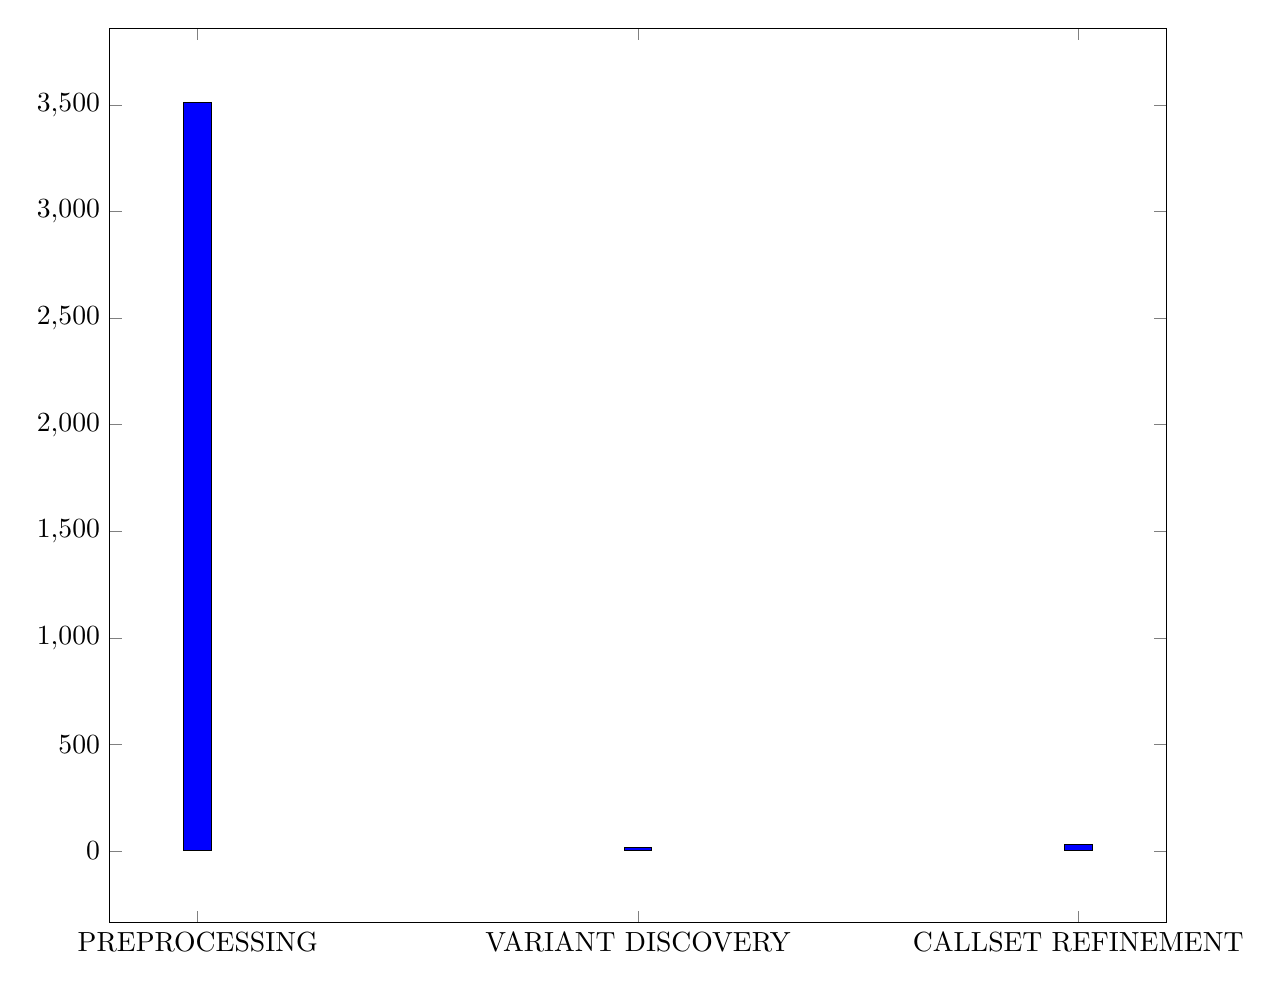
\begin{tikzpicture}
    \pgfplotsset{width=15cm,compat=1.9}
        \begin{axis}[
            symbolic x coords={PREPROCESSING, VARIANT DISCOVERY, CALLSET REFINEMENT},
            xtick=data
          ]
            \addplot[ybar,fill=blue] coordinates {
                (PREPROCESSING,   3511.7)
                (VARIANT DISCOVERY,  13.82)
                (CALLSET REFINEMENT,   31.37)
            };
        \end{axis}
    \end{tikzpicture}
\caption{Preprocessing, Variant Discovery and Call-set Refinement execution times with 6 input samples)}\label{cht:pvc}
\end{chart}

\begin{chart}[!ht]
\centering
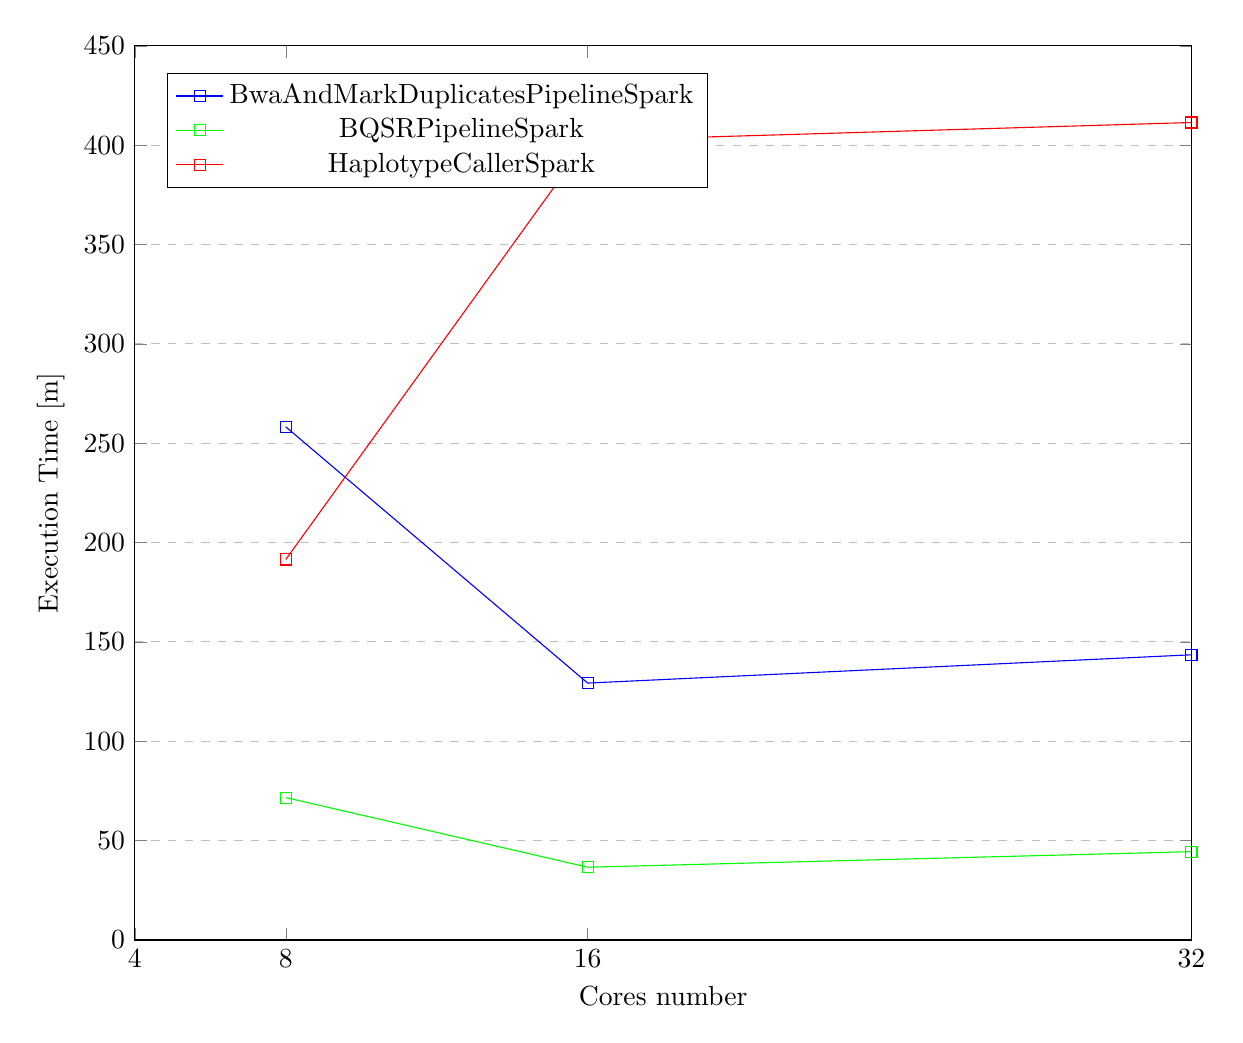
\begin{tikzpicture}
\pgfplotsset{width=15cm,compat=1.9}
\begin{axis}[
    title={},
    xlabel={Cores number},
    ylabel={Execution Time [m]},
    xmin=4, xmax=32,
    ymin=0, ymax=450,
    xtick={4,8,16,32},
    ytick={0,50,100,150,200,250,300,350,400,450},
    legend pos=north west,
    ymajorgrids=true,
    grid style=dashed,
]
 
\addplot[ color=blue, mark=square, ]
    coordinates {
    (8,258.23)(16,129.29)(32,143.52)
    };
\addplot[ color=green, mark=square, ]
    coordinates {
    (8,71.66)(16,36.62)(32,44.45)
    };
\addplot[ color=red, mark=square, ]
    coordinates {
    (8,191.49)(16,402.33)(32,411.4)
    %191.49 402,33
    };
\legend{BwaAndMarkDuplicatesPipelineSpark,BQSRPipelineSpark,HaplotypeCallerSpark}
\end{axis}
\end{tikzpicture}
\caption{Analysis performance variating the VM cores number (scale-up)}\label{cht:scale-up}
\end{chart}


\begin{chart}[!ht]
\centering
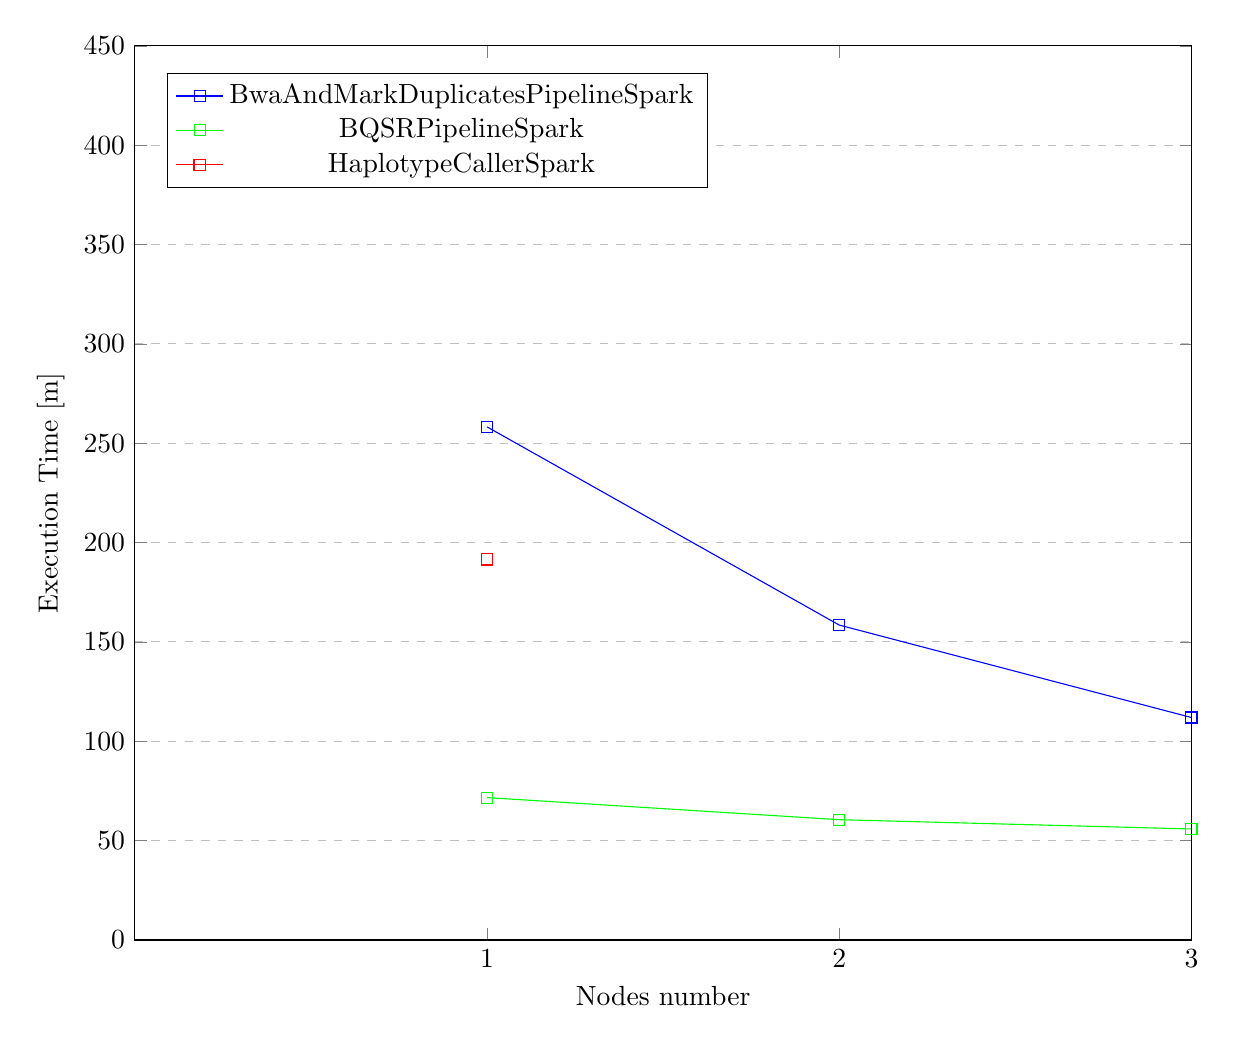
\begin{tikzpicture}
\pgfplotsset{width=15cm,compat=1.9}
\begin{axis}[
    title={},
    xlabel={Nodes number},
    ylabel={Execution Time [m]},
    xmin=0, xmax=3,
    ymin=0, ymax=450,
    xtick={1,2,3},
    ytick={0,50,100,150,200,250,300,350,400,450},
    legend pos=north west,
    ymajorgrids=true,
    grid style=dashed,
]
 
\addplot[ color=blue, mark=square, ]
    coordinates {
    (1,258.23)(2,158.48)(3,111.96)
    };
\addplot[ color=green, mark=square, ]
    coordinates {
    (1,71.66)(2,60.54)(3,55.87)
    };
\addplot[ color=red, mark=square, ]
    coordinates {
    (1,191.49)
    };
\legend{BwaAndMarkDuplicatesPipelineSpark,BQSRPipelineSpark,HaplotypeCallerSpark}
\end{axis}
\end{tikzpicture}
\caption{Analysis performance variating the nodes number (scale-out), where each node is a 8 cores 55 GB RAM VM}\label{cht:scale-out}
\end{chart}




















